% -*- coding: utf-8 -*-

\chapter{Introducción}

\section{Preámbulo}

La robótica móvil es un campo de investigación relativamente reciente que actualmente ocupa importantes líneas de trabajo en laboratorios y centros técnicos de todo el mundo. Su desarrollo supone la integración de numerosas disciplinas entre las que se encuentran la automática, la electrónica, la ingeniería mecánica, la informática, la inteligencia artificial, la estadística \ldots

Para ser considerado como tal, un robot móvil precisa de un sistema de locomoción que le permita desplazarse. Existen numerosas posibilidades al respecto, ya que podemos encontrar robots que andan, saltan, reptan o se mueven sobre ruedas y también robots aéreos o submarinos cuyo sistema motriz se basa en impulsion fluidomecánica. La mayor parte de estos mecanismos de locomoción surge como imitación de los modos de movimiento que se pueden observar en la naturaleza. La principal excepción es la rueda, ampliamente utilizada por sus buenas características sobre suelo plano.

Dentro de los robots móviles, los robots autónomos son aquellos que no necesitan la intervención humana para mantener el sentido de la orientación y la capacidad de navegación. Como indica Smithers, la idea principal del concepto de autonomía se obtiene de su etimología: \emph{auto} (propio) y \emph{nomos} (ley o regla). Los sistemas automáticos se autorregulan pero no son capaces de generar las leyes que deben tratar de seguir sus reguladores. A diferencia de ellos, los sistemas autónomos han de poder determinar sus estrategias, o leyes, de conducta y modificar sus pautas de comportamiento al mismo tiempo que operan en el entorno. Por lo tanto, queda claro que la autonomía añade requisitos sobre el concepto de automatismo.

Los robots autónomos deben ser capaces de adquirir información sobre el entorno. Para ello han de contar con sensores que proporcionen las medidas y datos necesarios. Aunque no son estrictamente imprescindibles, los robots móviles suelen incorporar sensores propioceptivos que suministran medidas relativas a su estado: velocidad, incremento de posición y aceleraciones. Los encoders situados en las ruedas del robot, por ejemplo, re\-gistran el número de revoluciones de las mismas y permiten obtener la llamada posición odométrica a partir de la estimación del movimiento relativo incremental. Aunque esta aproximación presenta una buena precisión a corto plazo, la acumulación de errores a medida que aumenta el recorrido causa grandes diferencias con la posición real. Por este y otros motivos hace falta disponer de sensores estereoceptivos para percibir los aspectos externos al robot. Los sensores de este tipo más comunes en robótica móvil avanzada son los de ultrasonidos, infrarrojos, los láseres y las cámaras.
Asimismo, el robot ha de poseer computadores o microprocesadores para el procesamiento de la información y la ejecución de los algoritmos de control del sistema de navegación.

Los robots móviles presentan la gran ventaja de poder emplear sus habilidades particulares allí donde sea necesario. Esta es la clave de su creciente demanda comercial. En los últimos años se han multiplicado sus aplicaciones en entornos industriales, militares, domésticos y de seguridad \cite{Arranz06}.

Algunos ejemplos de robots de este tipo son los cortacésped, los robots aspiradora, los \emph{Rovers} de Marte, los robots guía \ldots

Los robots cortacésped suelen utilizar algún medio que delimite la superficie a recorrer (como puede ser un cable que sirva de frontera para cerrar un recinto). Una vez señalada el área de césped a cortar, hacen un barrido irregular de toda la superficie.

\begin{figure}[hbt]
  % Requires \usepackage{graphicx}
  \centering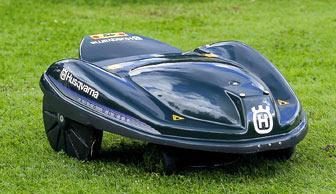
\includegraphics[width=0.4\textwidth]{Cortacesped}\\
  \caption{Robot cortacésped Automower Husqvarna}\label{fg:cortacesped}
\end{figure}

Los robots aspiradores son capaces de realizar la limpieza de todo tipo de suelos. Suelen constar de dos ruedas traseras motrices y una rueda delantera directriz. Hay modelos básicos que se mueven de forma aleatoria, sin cubrir normalmente la totalidad del espacio a limpiar, y modelos avanzados que incorporan las últimas técnicas de mapeo para lograr una alta eficiencia de funcionamiento.

\begin{figure}[h]
  % Requires \usepackage{graphicx}
  \centering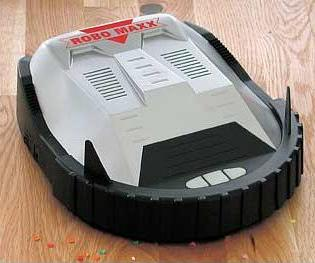
\includegraphics[width=0.4\textwidth]{aspirador}\\
  \caption{Robot aspirador RoboMaxx }\label{fg:aspirador}
\end{figure}

Los \emph{rovers} constan de un cuerpo central que se desplaza sobre seis ruedas y tienen una cabeza y un cuello para que las cámaras puedan tener una mejor perspectiva. Estas cámaras se utilizan para la construcción de mapas que les permitan guiarse por el territorio así como para enviar imágenes a la Tierra. Estos robots también cuentan con un un brazo robótico y un gran número de sistemas térmicos, además de los sistemas de baterías y de comunicaciones.

\begin{figure}[h]
  % Requires \usepackage{graphicx}
  \centering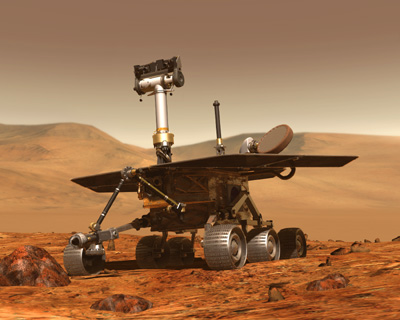
\includegraphics[scale=0.5]{MarsRover2}\\
  \caption{Rover sobre la superficie de Marte}\label{fg:rover}
\end{figure}

Los rovers \emph{Spirit} y su "gemelo" \emph{Opportunity} aterrizaron en el planeta rojo el 4 y el 25 de enero de 2004, respectivamente. Tienen una capacidad de movilidad mucho mayor que su antecesor el rover \emph{Pathfinder}.

Los robot guía son un tipo de robots móviles que han de tener amplio conocimiento sobre su entorno. Sus requisitos primordiales están orientados a la interacción con las personas, pero también es imprescindible en ellos un buen sistema de navegación que les permita desplazarse de forma autónoma en exposiciones, ferias y museos. Uno de estos robots es \emph{Urbano} (ver \ref{UrbanoProject}, \ref{Urbano}, Anexo B), un robot inteligente que ha sido empleado en el presente proyecto.

\section{Antecedentes}

En el grupo de Control Inteligente de la Universidad Politécnica de Madrid, en el cual se ha realizado este proyecto, trabaja un equipo de profesores e ingenieros con elevada experiencia en el campo de los robots móviles.

\subsection{Proyectos previos}
Los proyectos dentro de esta área que más significativamente han contribuido al nivel alcanzado se describen a continuación por orden de antigüedad. En la siguiente sección se describirá el hardware de los robots empleados.

\subsubsection{Panorama (1989-1993)}
Financiado por la Unión Europea (Proyecto ESPRIT 2483), consiste en la elaboración de un sistema avanzado de percepción y navegación para vehículos industriales dentro de entornos parcialmente estructurados y parcialmente conocidos. El proyecto estuvo orientado a demostrar la viabilidad de sistemas de transporte autónomos que pudieran sustituir a vehículos controlados por conductor en un amplio rango de aplicaciones.

\begin{figure}[hbt]
  % Requires \usepackage{graphicx}
  \centering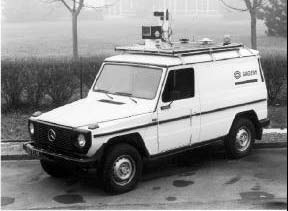
\includegraphics[width=0.5\textwidth]{Panorama}\\
  \caption{Proyecto Panorama}\label{fg:panorama}
\end{figure}


\subsubsection{RM-III (1994-1996)}
Sistema central de control para un sistema industrial de transporte basado en múltiples robots móviles autónomos dotados de inteligencia. Los vehículos tienen un alto grado de autonomía que les permite evitar obstáculos y buscar en cada caso el mejor camino a seguir. Los obstáculos pueden ser tanto fijos como móviles, con lo que la dificultad aumenta. Un componente adicional en la autonomía de los vehículos lo constituye su capacidad para gestionar el nivel de carga de sus baterías, trasladándose y conectándose automáticamente a los puntos de suministro de energía al considerarlo conveniente. Este proyecto fue financiado por la Comisión Interministerial de Ciencia y Tecnología y contó con la participación de UPM-DISAM y de la Universidad Carlos III.

\begin{figure}[hbt]
  % Requires \usepackage{graphicx}
  \centering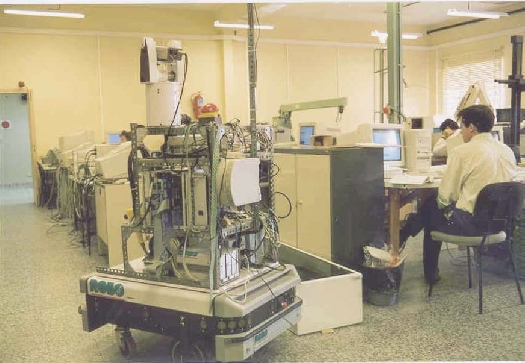
\includegraphics[width=0.5\textwidth]{Robotica3}\\
  \caption{Proyecto RM-III}\label{fg:RM-III}
\end{figure}


\subsubsection{EVS (1996-1999)}
Desarrollo de un entorno de ingeniería para facilitar el diseño y la implementación de sistemas autónomos distribuidos con aplicación en robótica móvil y en procesos continuos. Este entorno proporciona herramientas para el prototipado rápido y la experimentación, por medio de un sistema de realidad virtual que modela el sistema en desarrollo y su entorno.

\begin{figure}[hbt]
  % Requires \usepackage{graphicx}
  \centering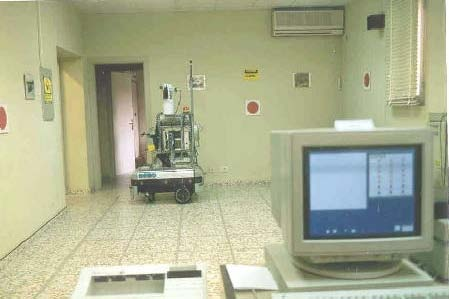
\includegraphics[width=0.5\textwidth]{EVS}\\
  \caption{Proyecto EVS}\label{fg:EVS}
\end{figure}


\subsubsection{Mobinet (1996-2000)}
Trabajo científico de un amplio conjunto de investigadores europeos en el diseño de un prototipo de robot móvil inteligente y completamente autónomo, con alta capacidad de maniobrabilidad y manipulación. Destinado a servir de ayuda a personas discapacitadas, la interacción con el usuario se lleva a cabo a través de comandos de muy alto nivel. El proyecto fue financiado por la Unión Europea bajo programa TMR (Training and Mobility of Researchers).

\begin{figure}[hbt]
  % Requires \usepackage{graphicx}
 \centering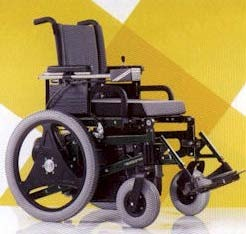
\includegraphics[scale=1.0]{MobiNet}\\
  \caption{Proyecto MobiNet}\label{fg:mobinet}
\end{figure}


\subsubsection{Blacky (2000-2001)}
Diseño de un prototipo de robot móvil para navegación en entornos parcialmente estructurados y con un elevado número de personas.El objetivo del proyecto es desarrollar un robot capaz de moverse en entornos complicados, tipo recintos feriales, e interaccionar con las personas que allí se encuentren.
Desde el punto de vista del control reactivo, los obstáculos no sólo no son fijos, sino que su movimiento es
totalmente imprevisible. Desde el punto de vista de la localización, se empleaba un sistema de marcas fijas en las paredes. El robot se encuentra con bastante frecuencia totalmente rodeado por personas, lo que complicaba la determinación de su posicionamiento.

\begin{figure}[h]
  % Requires \usepackage{graphicx}
  \centering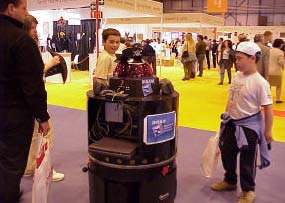
\includegraphics[width=0.5\textwidth]{Blacky}\\
  \caption{Proyecto Blacky}\label{fg:blacky}
\end{figure}


\subsubsection{WebFair (2001-2004)}
Proyecto Europeo Ref: IST-2000-29456.

Desarrollo y validación de un sistema de tele-presencia basado en robots móviles, capaz de facilitar el acceso de individuos a grandes exhibiciones y ferias comerciales a través de internet. La construcción de mapas y demás pruebas se realizaron en el Castillo de Belgioso, Italia, dedicado a la celebración de exposiciones.

\begin{figure}[h]
  % Requires \usepackage{graphicx}
  \centering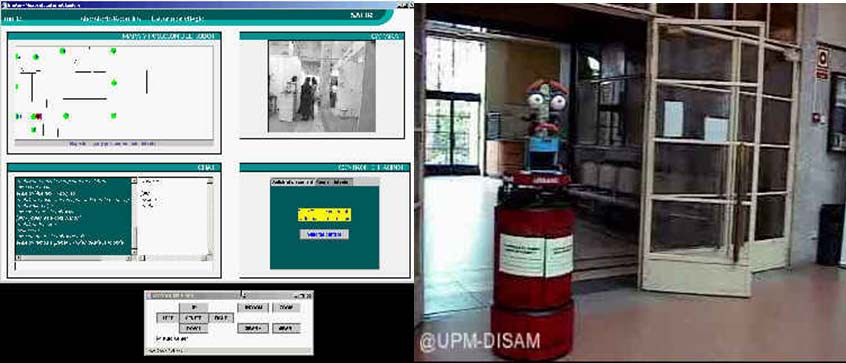
\includegraphics[width=0.5\textwidth]{WebFair}\\
  \caption{Proyecto WebFair}\label{fg:WebFair}
\end{figure}

\subsubsection{Guido (2004)}
Sistema de navegación robusto para un robot de la empresa Haptica que sirva de ayuda a la movilidad de personas débiles o con problemas de visión. Un punto a destacar entre las mejoras introducidas es la utilización de la información proporcionada por los bordes de segmentos del mapa, lo cual evita redundancias y permite así disminuir el coste computacional \cite{RodriguezLosada05}. Muy buenos resultados en casos reales empleando un ordenador portátil auxiliar.

\begin{figure}[h]
  % Requires \usepackage{graphicx}
  \centering\includegraphics[scale=0.8]{GuidoProject}\\
  \caption{Proyecto Guido}\label{fg:guido}
\end{figure}

\subsubsection{Urbano(2001-2004)}\label{UrbanoProject}
Proyecto de investigación nacional Ref: DPI2001-3652C0201.

Proyecto financiado por el Ministerio de Ciencia y Tecnología y supervisado por la Ciudad de las Artes y las Ciencias de Valencia (CACSA), donde el robot se ha probado con éxito. El módulo de navegación fue desarrollado por Diego Rodríguez-Losada en el marco de su Tesis Doctoral,\cite{Rodriguez-Losada04}

\begin{figure}[h]
  % Requires \usepackage{graphicx}
  \centering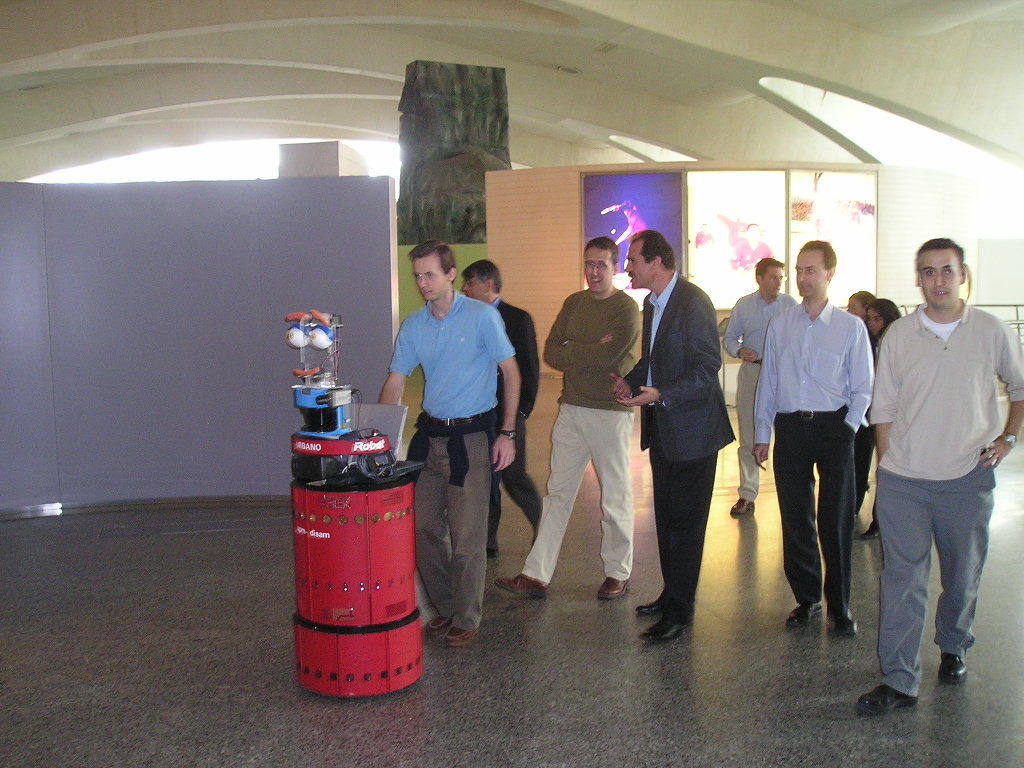
\includegraphics[width=0.5\textwidth]{UrbanoValencia}\\
  \caption{Proyecto Urbano}\label{fg:urbano}
\end{figure}

\clearpage
\subsubsection{RobInt (2004-2007)}
Ref: DOI 2004-007908C0201.

Modelado, diseño de una tecnología de diseño e implementación de comportamientos inteligentes en robots guía. Se trata de un proyecto financiado por el Ministerio de Ciencia y Tecnología que da continuidad al proyecto Urbano introduciendo mejoras en los módulos de navegación, consciencia y emociones, conocimiento y diálogo.

\subsection{Robots}
\subsubsection{ROBUTER}
Fabricado por Robosoft, consiste en una plataforma con elevada capacidad sensorial pensada para trabajo de experimentación. El modo de locomoción es diferencial y cuenta con un computador principal de Motorola con sistema operativo Albatros. Tiene también un computador secundario Sun Sparc. Los sensores de proximidad que posee son 24 sensores de ultrasonidos. También presenta capacidad de visión y Wireless Ethernet. Este robot se utilizó en los proyectos RM-III y EVS.

\begin{figure}[h]
  % Requires \usepackage{graphicx}
  \centering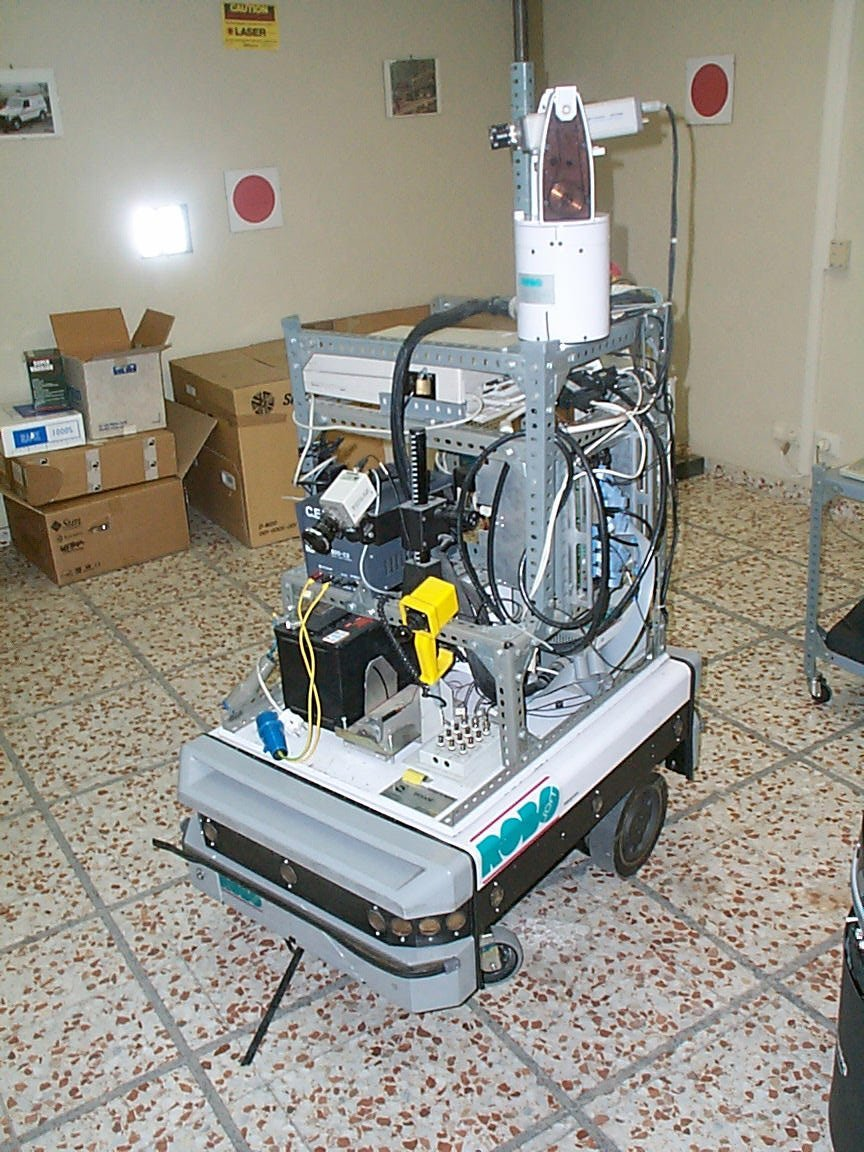
\includegraphics[scale = 0.2]{ROBUTER}\\
  \caption{Robot ROBUTER}\label{fg:robuter}
\end{figure}

\subsubsection{BLACKY}
Plataforma MRV-4 de Denning Branch Int. Robotics dotada de un PC Pentium con sistema operativo Linux y un láser rotatorio para la localización con balizas reflectantes. También posee 24 sensores de ultrasonidos y Ethernet Wireless radio. Es el robot utilizado en el proyecto del mismo nombre.

\begin{figure}[h]
  % Requires \usepackage{graphicx}
  \centering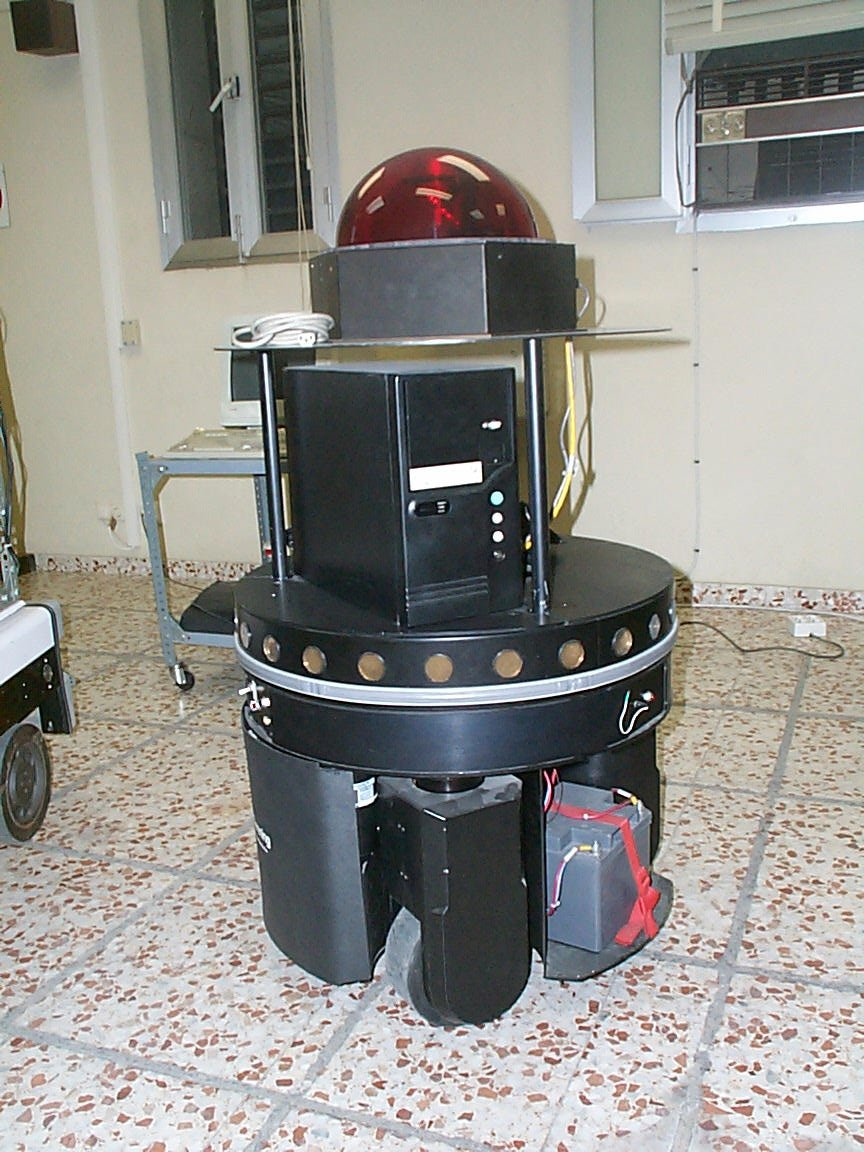
\includegraphics[scale = 0.2]{MRV-4}\\
  \caption{Robot BLACKY}\label{fg:mrv4}
\end{figure}

\subsubsection{URBANO}\label{Urbano}
Plataforma B21r del fabricante iRobot. El computador base es un PC Pentium con sistema operativo Linux; el computador secundario es un PC Pentium con Windows. Dispone de un láser SICK LM300 para la localización. También posee 24 sensores de ultrasonidos e infrarrojos y Ethernet Wireless radio. En DISAM-UPM se han desarrollado una cabeza y un brazo con los que el robot puede hacer gestos e interaccionar con personas. Este robot se ha empleado en los proyectos WebFair, Urbano y RobInt.

\begin{figure}[h]
  % Requires \usepackage{graphicx}
  \centering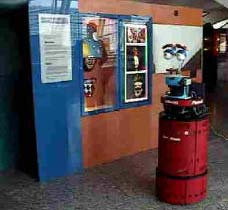
\includegraphics[scale=1]{Urbano}\\
  \caption{Robot Urbano}\label{fg:b21r}
\end{figure}

Dado que este robot ha sido asimismo utilizado en el desarrollo de este proyecto, puede consultarse más información sobre él en el Anexo B.

\subsubsection{GUIDO}
Guido es un robot de cuatro ruedas con dos motores para hacer girar las dos delanteras, pero ha de ser empujado para moverse \cite{Rodriguez-Losada05}. Tiene un sensor láser para percibir el entorno y en el manillar hay un sensor de medida de fuerza para detectar el comando de giro. El computador de a bordo es un PC104 300~MHz Geode con 32~MB de disco duro y 32~MB de RAM, con sistema operativo Haptica-TinyDCLinux. Tiene disponible un puerto Ethernet para las comunicaciones y se alimenta a 24V suministrados por cuatro baterías.

\begin{figure}[h]
  % Requires \usepackage{graphicx}
  \centering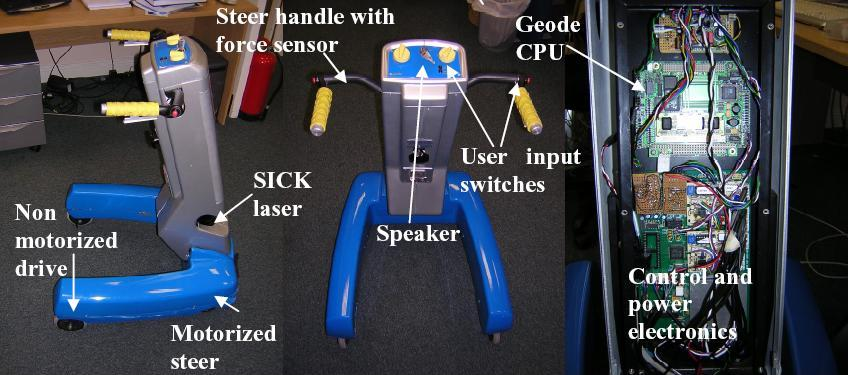
\includegraphics[scale=0.4]{Guido1}\\
  \caption{Robot Guido}\label{fg:guido}
\end{figure}


\section{Marco del proyecto}
Este proyecto se ha llevado a cabo bajo beca de colaboración concedida por el Ministerio de Educación y Ciencia en el Departamento de Automática, Ingeniería Electrónica e Informática Industrial de la Escuela Técnica Superior de Ingenieros Industriales de la Universidad Politécnica de Madrid, dentro del grupo de Control Inteligente.

\section{Objetivos del proyecto}
El objetivo del proyecto consiste en la realización de un sistema de navegación para un robot móvil. Se ha trabajado en control de movimiento, planificación de trayectorias, control reactivo, localización y construcción de mapas.

\section{Alcance del proyecto}
Los principales elementos de trabajo en este proyecto son los siguientes:
\begin{itemize}
  \item \textbf{Formación previa.} En primer lugar se requería un asentamiento de conocimientos sobre programación y algorítmica, el aprendizaje de C++ y Visual C++. Posteriormente fue necesaria la comprensión de la base de software de navegación existente. Otra parte importante era la puesta en funcionamiento del robot Pioneer P3AT y el estudio de las librerías de la distribución Aria.
  \item \textbf{Desarrollo del control de movimiento.} Programación de un regulador proporcional con planificación de ganancia, empleando tanto los parámetros de Urbano como los correspondientes al Pioneer. Generación de una trayectoria suave en los puntos de paso de una trayectoria definida. Algoritmo para evitar desviaciones sobre la trayectoria programada. Control reactivo: deformación de la trayectoria por la presencia de obstáculos y paredes cercanas al camino inicial a seguir por el robot.
  \item \textbf{Localización y construcción de mapas.} Estudio del filtro de Kalman y del filtro extendido de Kalman (EKF). Aplicación a la la localización del robot a partir de los puntos de medida proporcionados por el láser. Modificación del modelo para el caso de disponer únicamente de medidas de distancia, que no se utiliza debido a su peor comportamiento. Programación de las fases de predicción y corrección del algoritmo. Análisis del coste computacional y reducción del tiempo de procesamiento. Obtención y actualización de mapas de puntos a partir de los datos registrados por el láser. Utilización de mapas ya realizados para efectuar la localización. Borrado de los puntos correspondientes a obstáculos dinámicos del mapa que se encuentren cercanos a la posición del robot en cada momento.
      Con el Pioneer sólo es utilizable la parte del proyecto relativa al control de movimiento, planificación de trayectorias y control reactivo ya que al no poderse utilizar el láser no era posible realizar tareas de localización.
  \item \textbf{Integración.} Funcionamiento conjunto e intercambio de información entre los componentes anteriormente indicados.
  \item \textbf{Pruebas.} Pruebas de funcionamiento en modo simulación y con los robots reales. Corrección, depuración y posibles mejoras a partir de los resultados de dichas pruebas.

  Paralelamente se iba desarrollando un cuadro de diálogo para facilitar la ejecución y la selección de opciones en la misma.
\end{itemize}
